\section{Project Vision}
%A representation of your Project Vision and (if relevant) Prospect Research (see Essence-book Chapter 15).
%Explain your choice of representation type (see Essence-book Chapter 24).
The \textit{Project Vision}, according to \citet[ p. 104]{essence}, is used to outline a common goal and keep the project on track, while still allowing it to adapt to changes and ambiguities.
For this application we chose the metaphor \texttt{paser}. A metaphor citep[ pp. 172-174]{essence} has to be interpreted and coveys only part of the idea. In our application the metaphor can be interpreted both as setting the music tempo after runners pace and as setting runners pace after music tempo. 

\noindent \textit{Prospect Research} is about researching problems and their solutions to gain enough knowledge to be able to solve them, if this knowledge is not already available in the team \citep[ pp. 104-105]{essence}.
Prospect research has been widely used in this project, and the following are some of the questions we tried to answer:

\begin{itemize}
	\item Is is possible to use music to influence peoples' running style and/or intensity?
	\item Is is possible to reliably measure the user's pace using the accelerometer?
	\item Can we find a way to manage starting and stopping music based on this data, without disrupting the flow of the application?
\end{itemize}

While prospect research takes time, it also allowed us to focus on solving tasks that were feasible, helping us reduce time spent on trying to solve problems that are too hard or irrelevant for the Vision.

\subsection*{Vision Scenarios}
%Characterization of your project using Vision Scenarios  (see Essence-book Part 4):
	% Describe your axes.
For our vision scenarios \cite[ p. 127]{essence} we have selected the following dimensions:
\begin{itemize}
\item Online vs. Offline %Client Server vs Standalone
\item Narrow vs. Wide
\end{itemize}

The \texttt{Online vs. Offline} dimension points to variations in reliance on online resources. An online focus could shift  towards a server with a thin client application. Music streaming comes to mind, which would allow a large music libary to be available on the smartphone. A drawback of a shift towards online is that it requires a stable internet connecting. An offline standalone application would rely on a local music libary and not be dependant on a stable internet connection in order to function. It would however be more difficult to acquire not commonly used information from local music files such as beat pr minute.

The \texttt{Narrow vs. Wide} dimension points to variations in scope of the application. A narrow scope will result in a focused application covering just running, but supports more running related features. One the other hand a wider scope will cover more general forms of exercise. For a user performing multiple forms of exercise there might a benefit to having everything linked in the same application, even if it is at the cost of more specialised features. Another drawback of the multi purpose application is that it might be harder to operate.


	%Characterize the project using at least one of the Essence roles.

From these dimensions we can identify four vision scenarios based on the child role  \cite[ pp. 132-134]{essence}, as seen in figure \Cref{fig:axis1}

\begin{figure}[h!]
  \centering
    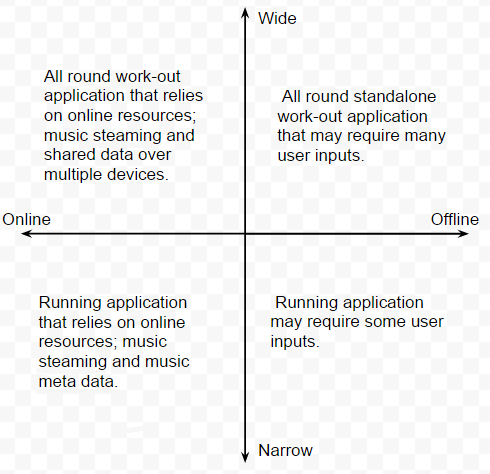
\includegraphics[width=0.6\textwidth]{Images/axis1.PNG}
    \caption{Vision scenario for the application.}
    \label{fig:axis1}
\end{figure}

%\begin{itemize}
%\item Running application that relies on online resources; music steaming and music meta data. %Online - Narrow
%\item All round work-out application that relies on online resources; music steaming and shared data over multiple devices. %Online - Wide
%\item Running application may require some user inputs. %Offline - Narrow
%\item All round standalone work-out application that may require many user inputs. %Offline - Wide
%\end{itemize}

The challenger role can contribute the vision scenarios taking the customer's wishes into consideration. These features ideas can be seen in \Cref{fig:axis2}.
%\begin{itemize}
%\item A well thought through running assistant. Stable/reliable online resources (e.g. web service).%Online - Narrow
%\item Many workout options/programs. Stable/reliable online resources (e.g. web service). %Online - Wide
%\item A well thought through running assistant. Easy data input.  %Offline - Narrow
%\item Many workout options/programs. Many user settings. Easy data input.  %Offline - Wide
%\end{itemize}

\begin{figure}[h!]
  \centering
    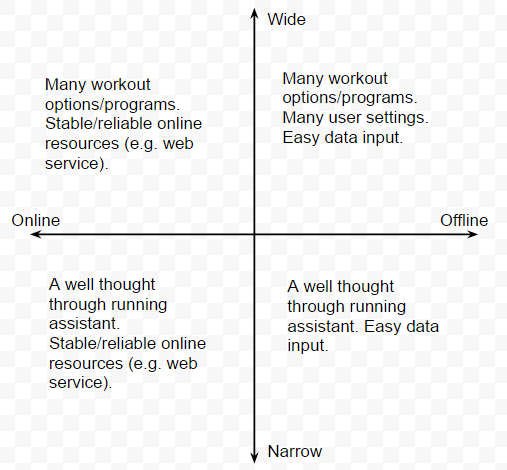
\includegraphics[width=0.6\textwidth]{Images/axis2.PNG}
    \caption{Features ideas for the challenger role's contribution to the vision scenarios.}
    \label{fig:axis2}
\end{figure}
